%%=============================================================================
%% Methodologie
%%=============================================================================

\chapter{Methodologie}
\label{ch:methodologie}

%% TODO: Hoe ben je te werk gegaan? Verdeel je onderzoek in grote fasen, en
%% licht in elke fase toe welke stappen je gevolgd hebt. Verantwoord waarom je
%% op deze manier te werk gegaan bent. Je moet kunnen aantonen dat je de best
%% mogelijke manier toegepast hebt om een antwoord te vinden op de
%% onderzoeksvraag.

Om een antwoord te vinden op de gestelde onderzoeksvragen dient er een experiment uitgevoerd te worden. Hoe dit experiment zal verlopen wordt hieronder nader verklaard.

\section{Plan van aanpak}

Het experiment zal grotendeels uitgevoerd worden op willekeurige testpersonen. Bij deze testpersonen zal er a.d.h.v. een wasknijper een pijnprikkel opgewekt worden. Deze pijnprikkel zal gedurende enkele oefensessies verdragen moeten worden.

Bij een eerste oefensessie zal de persoon 10 maal een beweging moeten uitvoeren met de wasknijper op de vinger. 
Tijdens de tweede oefensessie zal de persoon de VR bril en een hoofdtelefoon opgezet krijgen. Hier zal hij terechtkomen in 'ApplePicker', het gerealiseerde prototype voor dit onderzoek. In deze game zal de persoon opnieuw 10 maal een beweging moeten uitvoeren, met de wasknijper op de vinger.

Na elke oefensessie dient de persoon een vragenlijst in te vullen 
over zaken zoals: hoe de pijnervaring was tijdens de oefeningen, of de persoon zich altijd even gemotiveerd voelt om revalidatie oefeningen uit te voeren, ...

Ook zal er een experiment uitgevoerd worden op enkele testpersonen die momenteel lijden aan een letsel aan de bovenste ledematen. Opnieuw zullen er enkele oefensessies plaatsvinden, maar nu onder begeleiding van de kinesist.

Gedurende de eerste oefensessie zal de kinesist de testpersoon bijstaan bij het uitvoeren van de oefeningen zonder enige hulp van VR.
Bij de tweede oefensessie zal de persoon dan opnieuw de VR bril en de hoofdtelefoon opgezet krijgen. Deze keer zal de kinesist de bewegingen van de patiënt op het computerscherm kunnen volgen om mogelijke instructies te kunnen geven. Wanneer de kinesist dit wenst zijn er ook polsgewichten om de oefeningen wat uitdagender te maken voor de patiënt.

Ook hier zal de persoon nadien nog een vragenlijst moeten invullen.

\chapter{Experiment}

\section{Materiaal}
Om het experiment uit te voeren waren enkele zaken onmisbaar:

- VR headset en controller: Hier werd de Oculus Go gebruikt

- Hoofdtelefoon: Dit zou de persoon nog meer moeten afsluiten van de realiteit

- Computer: Hierop werden de vragenlijsten ingevuld na de oefensessies. Ook kon de kinesist/begeleider hierop meevolgen wat de patiënt in het spel aan het doen was.

- Polsgewichten (eventueel): Deze konden bij de patiënt omgedaan worden om de intensiteit van de oefeningen te vergroten.

\newpage
\subsection{Testpersonen}
Als testpersonen werden er 25 willekeurige personen gekozen tussen de 19 en 85 jaar. Op \cite{figuur 6.1} kan u bijhorende boxplot terugvinden die een beeld geeft van de verdeling van de leeftijden per geslacht. De testpersoon werd op voorhand niet ingelicht over de opzet van het onderzoek. Dit om de onbevooroordeeldheid zo veel mogelijk te beperken.

\begin{figure}[h]
    \centering
    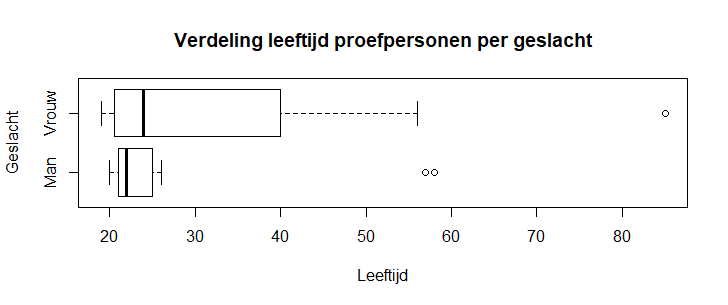
\includegraphics[scale=0.7]{Boxplot_Leeftijd.png}
    \caption{Boxplot van leeftijden van proefpersonen}
\end{figure}

Gedurende het experiment werd de proefpersoon een wasknijper opgedaan om een pijnprikkel op te wekken. Hierna diende de oefening uitgevoerd te worden (\cite{figuur 6.2}).

\begin{figure}[h]
    \centering
    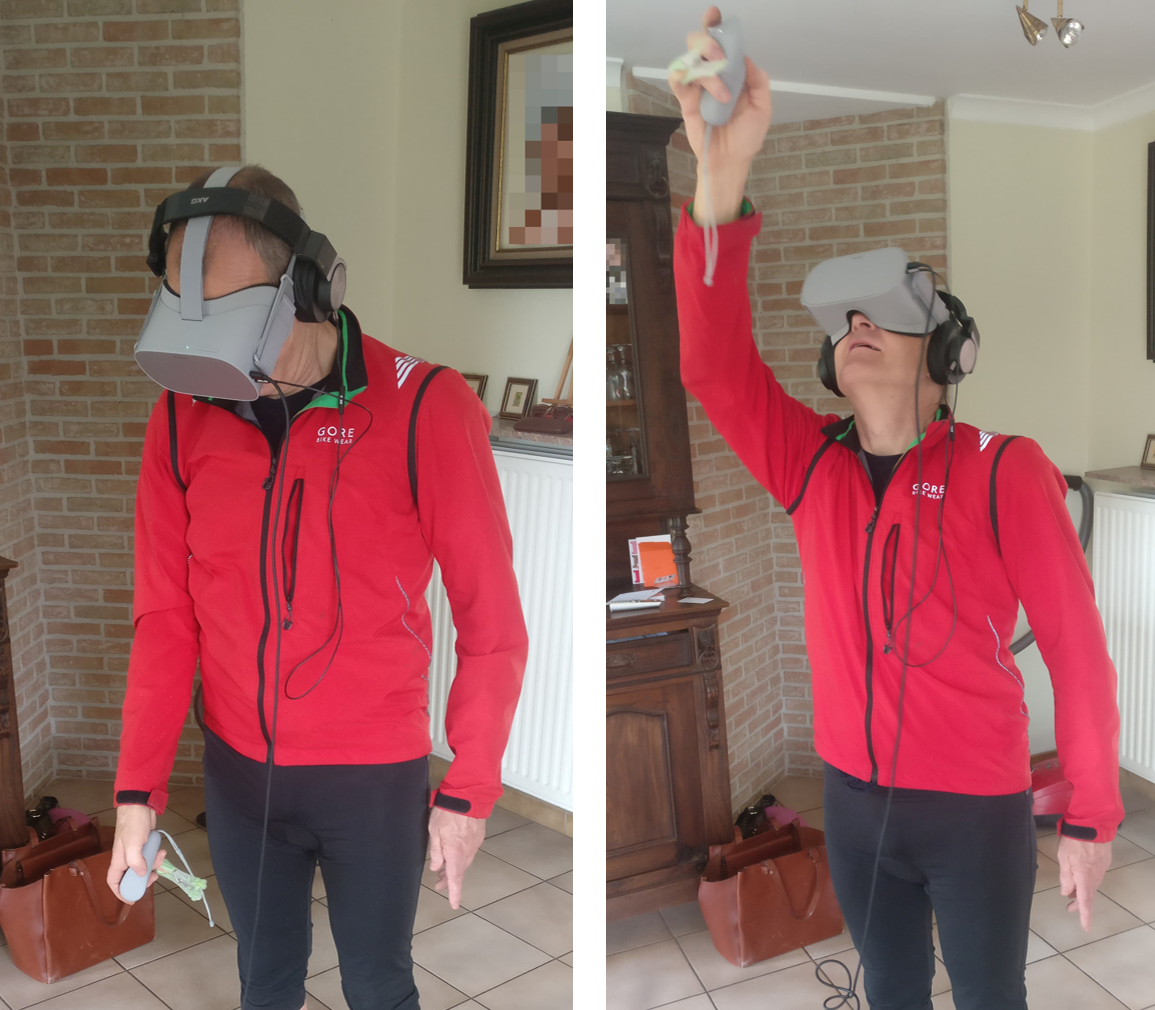
\includegraphics[scale=0.8]{luc.png}
    \caption{Proefpersoon test de applicatie met wasknijper op de vinger en voert de beweging uit}
\end{figure}

\newpage

\section{Resultaten}
Iedere persoon die zich onderwierp aan het experiment diende enkele vragenlijsten in te vullen. Onderstaande grafieken werden uit deze data geëxtraheerd.

\begin{figure}[h]
    \centering
    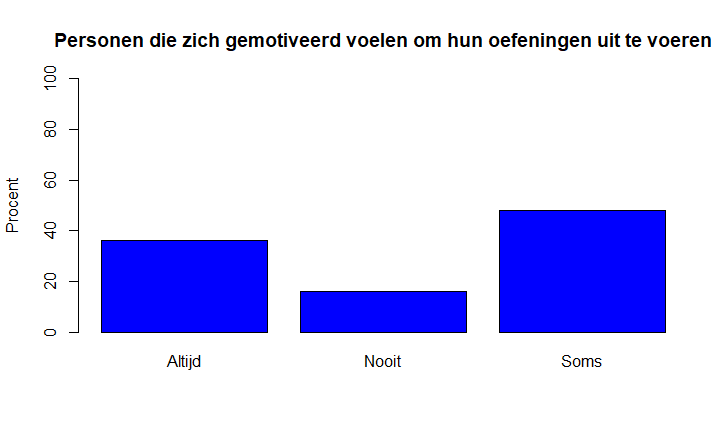
\includegraphics[scale=0.6]{barplot_motivatie.png}
    \caption{In welke mate men gemotiveerd is om consistent de revalidatie oefeningen uit te voeren}
\end{figure}

Bovenstaande grafiek (\cite{Figuur 6.3}) toont duidelijk dat mensen zich niet altijd gemotiveerd voelen om hun revalidatie oefeningen uit te voeren. Zo blijkt dat slechts 36\% van de personen zich altijd gemotiveerd voelt en 16\% zich nooit echt gemotiveerd voelt. 48\% voelt zich dan weer soms gemotiveerd om hun oefeningen uit te voeren.

\begin{figure}[h]
    \centering
    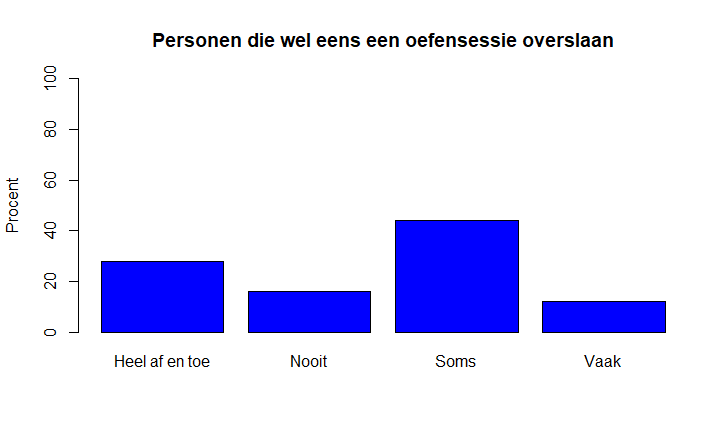
\includegraphics[scale=0.6]{barplot_overslaan.png}
    \caption{In welke mate oefensessies worden overgeslagen}
\end{figure}

Door het gebrek aan motivatie dat bij sommmigen wel eens de kop op steekt durft men dan ook hier en daar eens een oefensessie over te slaan (\cite{Figuur 6.4}). 28\% geeft toe dat ze af en toe hun oefeningen overslaan en 44\% soms wel eens. Hiernaast zijn er ook zeer gedreven mensen die nooit een sessie overslaan (16\%) en die het vaak overslaan (12\%).

\begin{figure}[h]
    \centering
    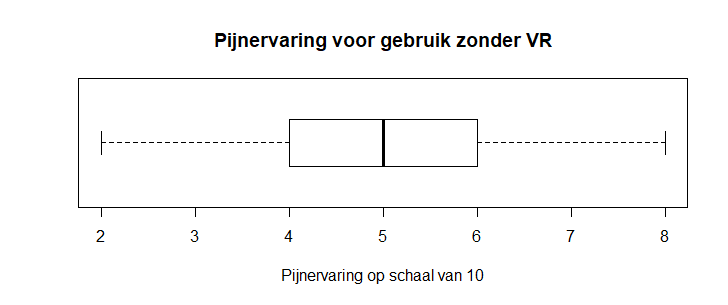
\includegraphics[scale=0.7]{boxplot_PijnZonder.png}
    \caption{Pijnervaring testgebruikers bij oefensesie zonder VR}
\end{figure}

Uit \cite{Figuur 6.5} kan men een mediaan van 5, een interkwartielafstand van 2 en een spreidingbreedte van 6 vaststellen.

\begin{figure}[h]
    \centering
    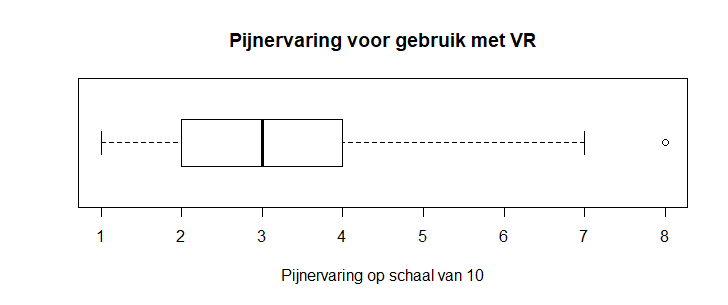
\includegraphics[scale=0.7]{boxplot_PijnMet.png}
    \caption{Pijnervaring testgebruikers bij oefensesie met VR}
\end{figure}

Uit \cite{Figuur 6.6} kan men een mediaan van 3, een interkwartielafstand van 2 en een spreidingsbreedte van 7 vaststellen.

Hier kan men dus concluderen dat op een paar uitschieters na, de pijnervaring bij iedereen significant gedaald was. Wanneer men de gemiddelde afname in pijn berekent komt men uit op een waarde van 1.88 op een schaal van 10 ofwel 18.8\%.

\begin{figure}[h]
    \centering
    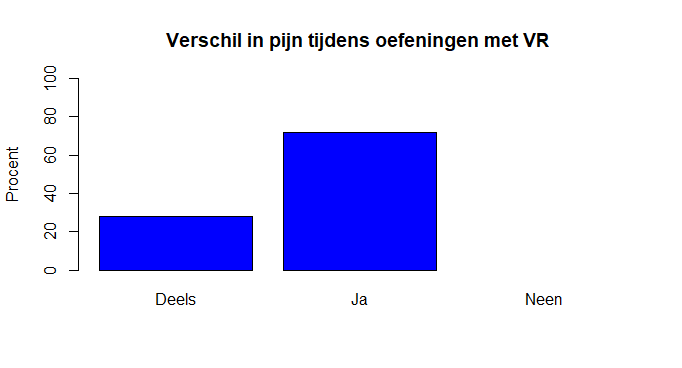
\includegraphics[scale=0.7]{barplot_verschilPijn.png}
    \caption{Diagram van verschil in pijnervaring die de proefpersonen ondervonden met en zonder VR}
\end{figure}

\newpage

Opnieuw wordt er in \cite{Figuur 6.7} bevestigd dat er wel degelijk een verschil in pijn werd waargenomen bij de testpersonen. Zo'n 72\% zegt dat er inderdaad een verschil is in pijn wanneer men de oefening met VR uitvoert. 28\% van de mensen merkten echter slechts deels een verschil.

\begin{figure}[h]
    \centering
    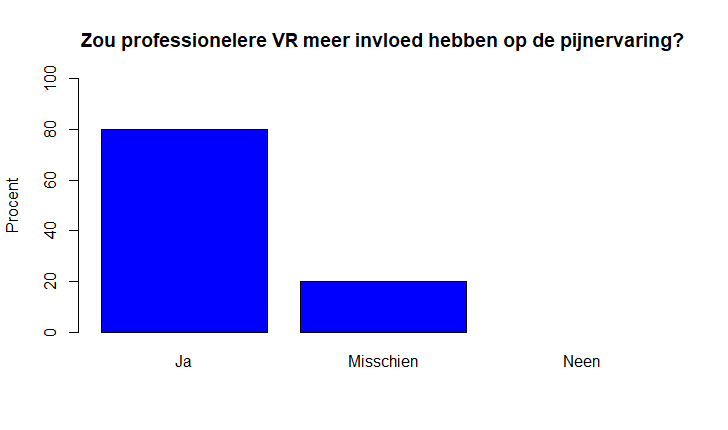
\includegraphics[scale=0.7]{barplot_profVr.png}
    \caption{Diagram van personen die denken dat professionelere VR meer invloed zou hebben op pijnervaring}
\end{figure}

In de grafiek op \cite{Figuur 6.8} merkt men dat velen ervan overtuigd waren dat het verschil in pijn nog significanter zou zijn tijdens het gebruik van gesofisticeerdere VR systemen (vrij bewegen in de ruimte, dynamischere omgeving, hogere kwaliteit, ...). 80\% van de testpersonen stemde hier volop mee in en 20\% zag de mogelijkheid ervan in.

\begin{figure}[h]
    \centering
    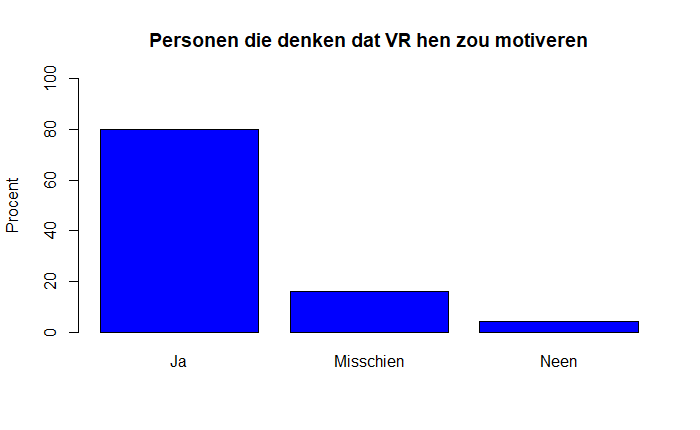
\includegraphics[scale=0.65]{barplot_extraMotivatie.png}
    \caption{Diagram van personen die geloven dat VR voor extra motivatie kan zorgen}
\end{figure}

Op \cite{Figuur 6.9} ziet men dat een groot aandeel zich meer gemotiveerd zou voelen om zijn oefeningen uit te voeren wanneer ze toegang zouden hebben tot een VR systeem. Opnieuw 80\% van de testpersonen zou zich meer gemotiveerd voelen, 16\% zou zich misschien meer gemotiveerd voelen en 4\% helemaal niet.

\begin{figure}[h]
    \centering
    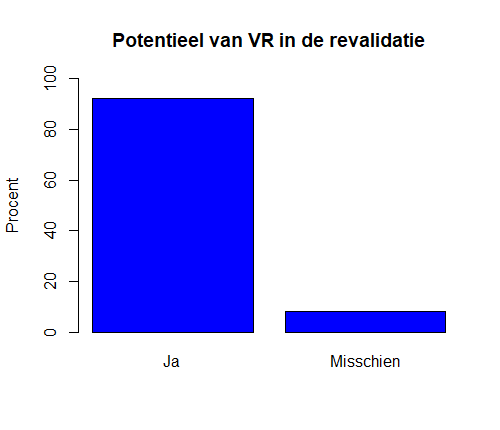
\includegraphics[scale=0.65]{barplot_potentieel.png}
    \caption{Diagram van personen die geloven dat VR potentieel heeft in de revalidatie}
\end{figure}

Tenslotte kan men uit \cite{Figuur 6.10} vaststellen dat er 92\% van de testpersonen echt wel potentieel ziet in het gebruik van VR tijdens de revalidatie. 8\% van de personen heeft hier echter nog wat twijfels bij.




